\documentclass[conf]{new-aiaa}
\usepackage[utf8]{inputenc}

\usepackage{graphicx}
\usepackage{amsmath}
\usepackage{siunitx}
\usepackage{float}
\usepackage{longtable,tabularx}
\usepackage{multirow, multicol}
\usepackage{minted}
\usepackage{verbatim}
\usepackage{lscape}
\usepackage[ruled,vlined]{algorithm2e}

% From https://tex.stackexchange.com/questions/323297/
\newcommand{\rvline}{\hspace*{-\arraycolsep}\vline\hspace*{-\arraycolsep}}

\graphicspath{{../../../plots}}

\usepackage{hyperref}
\renewcommand\refname{}
\urlstyle{same}
\hypersetup{
    colorlinks=false,
    linkcolor=black,
    filecolor=black,      
    urlcolor=cyan,
}

\title{Exploring Periodic Computation and Invariant Manifolds \\ within the Circular Restricted Three-body Problem}

\author{Joseph D. Carpinelli
    \footnote{
        M.S. Candidate, 
        Department of Aerospace Engineering, 
        University of Maryland, College Park}}

\begin{document}

\maketitle

\begin{abstract}
    Periodic orbits within the Circular Restricted Three-body Problem 
    (CR3BP) are more difficult to find than periodic orbits within the 
    Restricted Two-body Problem (R2BP). While any  elliptical or circular 
    R2BP orbit is periodic, the periodic subset of CR3BP orbits is far 
    more selective. Periodic CR3BP orbit-finding algorithms 
    have been known for decades, but their implementations are not easily
    found in free and open-source software -- the few implementations
    which do exist in free and open-source software don't hold 
    \textit{generally}. Instead, publicly accessible implementations may 
    find periodic orbits for one particular CR3BP system (e.g. Sun-Earth), 
    or  may find periodic orbits which have non-zero z-amplitudes. 
    General solutions for periodic CR3BP orbits are incredibly useful, as 
    CR3BP analysis is can be used as an approximate starting-point during 
    mission design. Invariant manifolds about periodic 
    CR3BP orbits can provide low-cost interplanetary transfers when 
    compared with traditional transfer designs. This paper introduces 
    a periodic CR3BP orbit-finding implementation that ties together
    known methods and existing code implementations; as a result, 
    this implementation works \textit{generally}. The numerical Halo 
    orbit solver is used to highlight several
    Halo orbit families in familiar CR3BP systems, and calculate invariant 
    manifolds about Halo orbits. Interplanetary manifold-based transfer
    designs are explored, and challenges that inhibit methods for 
    finding intersections are presented. All source code 
    is available on GitHub as part of 
    \textit{GeneralAstrodynamics.jl}, an astrodynamics package written 
    with the Julia programming language.
\end{abstract}

\begin{multicols}{2}

\tableofcontents

\section{Nomenclature}
\begin{flushleft}
\begin{tabularx}{\columnwidth}{ccl}
    $\overrightarrow{r}$ & $=$ & Spacecraft position \\
    $\overrightarrow{v}$ & $=$ & Spacecraft velocity \\
    $\Phi_m$             & $=$ & Monodromy matrix \\
    $\Phi$               & $=$ & State transition matrix \\
    R2BP                 & $=$ & Restricted Two-body Problem \\
    CR3BP                & $=$ & Circular Restricted Three-body Problem \\
    $S_L \triangleq a$   & $=$ & Distance between CR3BP bodies \\
    $S_T$                & $=$ & Time scale factor \\
    $\mu^\star$          & $=$ & Normalized CR3BP mass parameter \\
    $\overrightarrow{r}^\star$ & $=$ & Normalized spacecraft position \\
    $\overrightarrow{v}^\star$ & $=$ & Normalized spacecraft velocity \\
    $\overrightarrow{a}^\star$ & $=$ & Normalized spacecraft acceleration \\
    $r_i$                & $=$ & Nondimensional $x$ position of $i_{\text{th}}$ body \\ 
    $H$                  & $=$ & CR3BP potential energy Hessian matrix\\ 
    $M$                  & $=$ & Monodromy matrix\\     
\end{tabularx}
\end{flushleft}

\section{Introduction}
As space exploration targets shift from Earth's moon to Mars and 
beyond, low-cost trajectory designs are increasingly important 
\cite{nasa2020artemis}. One such family of low-cost trajectory 
designs utilizes invariant manifolds about Lagrange points
\cite{rund2018interplanetary}. Halo orbits can be estimated 
analytically with an expansion, as originally shown by Richardson 
\cite{richardson1980analytical} \cite{koon2008dynamical}. A known
numerical algorithm can iterate on non-periodic initial Halo orbit 
conditions to produce numerically periodic Halo orbits
\cite{howell1984three}. When placed in series, these two algorithms 
provide a proverbial \textit{black box} for astrodynamicists: 
given desired physical features (orbit amplitude, phase, etc.), 
the analytical algorithm can produce a Halo orbit estimate for the
numerical algorithm to iterate on \cite{rund2018interplanetary}.
These algorithms were recently implemented with the Julia 
programming language \cite{carpinelli2020halos} 
\cite{carpinelli2020astro} \cite{bezanson2017julia}. 

This paper presents technical and implementation details, lessons learned,
and periodic orbit and manifold results for common CR3BP systems in 
our solar system. 
First, an overview of the Circular Restricted Three-body Problem,
and periodic CR3BP orbits, is provided. Methods for calculating
periodic CR3BP orbits are briefly discussed, and a Julia 
implementation is introduced. 

Next, a short catalog of Sun-Earth, Sun-Mars, and Sun-Jupiter 
Halo orbits is presented using the developed Halo solvers.
This catalog will provide parameters for each Halo orbit, 
and initial conditions and orbital periods from which to propagate.
These catalogues orbits may be a helpful reference for future 
engineers who wish to explore periodic orbits within CR3BP dynamics
with applications in low-cost mission design.

Visualizations for stable and unstable 
manifolds near each chosen Halo orbit are shown. Points along the 
Halo orbits' stable manifolds are found, and 
transfers between LEO and these stable manifolds are defined. 
These manifolds are then used to generate interplanetary 
transfers. Methods and challenges relating to manifold-based 
transfer design are presented and discussed. 

All code written for this project is included in the open-source 
Julia package titled \textit{GeneralAstrodynamics.jl} \cite{carpinelli2020astro}.
A Pluto (Jupyter-like) notebook with code examples, and an informal 
project summary is provided 
\cite{fosnp2020Pluto} \cite{carpinelli2020halos}.

\section{CR3BP Overview}
The Circular Restricted Three-body Problem is a simplified 
dynamical model of an infinitesimally small spacecraft traveling
near two finite-mass celestial bodies. All masses are described
as point masses. The system's barycenter is the 
center of mass of the two celestial bodies, and both celestial 
bodies are constrained to travel in a circle about an inertial 
frame placed at the system barycenter. CR3BP spacecraft dynamics are 
typically described in the \textit{Synodic} frame, which is placed
at the barycenter of the system, and rotates about its Z axis such 
that each celestial body is fixed on the Synodic X axis. 
CR3BP spacecraft dynamics are also typically described with 
normalized units,
as shown in equations $\left(1\right)$ $\left(2\right)$ $\left(3\right)$
$\left(4\right)$. Normalized equations of motion for a spacecraft 
within the CR3BP are shown in equations 
$\left(5\right)$ $\left(6\right)$ $\left(7\right)$ $\left(8\right)$
$\left(9\right)$. Note that $\mu_2 \leq \mu_1$ by definition.

\subsection*{Normalized Synodic CR3BP State}
\begin{align}
    \mu^\star & = \frac{\mu_2}{\mu_1+\mu_2} \\
    S_t & = \sqrt{\frac{a^3}{\mu_1+\mu_2}} \\
    \overrightarrow{r}^\star & \triangleq \begin{bmatrix} x^\star & y^\star & z^\star \end{bmatrix}^T  = \frac{1}{S_L} \overrightarrow{r} \\
    \overrightarrow{v}^\star & \triangleq \begin{bmatrix} \dot{x}^\star & \dot{y}^\star & \dot{z}^\star \end{bmatrix}^T  = \frac{1}{S_T} \overrightarrow{v}
\end{align}

\subsection*{Normalized Synodic CR3BP Dynamics}

\begin{align}
    r_1 & = \sqrt{(x^\star+\mu^\star)^2 + (y^\star)^2 + (z^\star)^2} \\
    r_2 & = \sqrt{(x^\star+\mu^\star-1)^2 + (y^\star)^2 + (z^\star)^2} \\
    \ddot{x}^\star & = 2\dot{y}^\star + x^\star - \frac{(1-\mu^\star)(x^\star + \mu^\star)}{r_1^3} - 
        \frac{\mu^\star (x^\star - 1 + \mu^\star)}{r_2^3} \\
    \ddot{y}^\star & = -2\dot{x}^\star + y^\star - \frac{(1 - \mu^\star)y^\star}{r_1^3} - \frac{\mu^\star y^\star}{r_2^3} \\
    \ddot{z}^\star & = -\frac{(1-\mu^\star)z^\star}{r_1^3} - \frac{\mu^\star z^\star}{r_2^3} \\
    \dot{\Phi} & = \begin{bmatrix} I_{3 \times 3} & 0_{3 \times 3} \\ H \triangleq \frac{\partial^2 U}{\partial \overrightarrow{r}^2} & \begin{bmatrix} 0 & 2 & 0 \\ -2 & 0 & 0 \\ 0 & 0 & 0 \end{bmatrix} \end{bmatrix} \Phi
\end{align}

\begin{equation}
    \begin{aligned}
        H_{11} &= 1 - \frac{\mu}{r_2^{3}} - \frac{\left( 1 - \mu \right)}{r_1^{3}} + \frac{\frac{3}{4} \left( -2 + 2 x^{\star} + 2 \mu \right)^{2} \mu}{r_2^{5}} \\
        &- \frac{\frac{3}{2} \left(  - x^{\star} - \mu \right) \left( 2 x^{\star} + 2 \mu \right) \left( 1 - \mu \right)}{r_1^{5}}
    \end{aligned}
  \end{equation}

    
\begin{equation}
    H_{12} = \frac{\frac{3}{2} y^{\star} \mu \left( -2 + 2 x^{\star} + 2 \mu \right)}{r_2^{5}} - \frac{3 y^{\star} \left(  - x^{\star} - \mu \right) \left( 1 - \mu \right)}{r_1^{5}}
\end{equation}
    
    
\begin{equation}
    H_{13} =\frac{\frac{3}{2} z^{\star} \mu \left( -2 + 2 x^{\star} + 2 \mu \right)}{r_2^{5}} - \frac{3 z^{\star} \left(  - x^{\star} - \mu \right) \left( 1 - \mu \right)}{r_1^{5}}
\end{equation}
    
    
\begin{equation}
    H_{21} =\frac{\frac{3}{2} y^{\star} \mu \left( -2 + 2 x^{\star} + 2 \mu \right)}{r_2^{5}} - \frac{3 y^{\star} \left(  - x^{\star} - \mu \right) \left( 1 - \mu \right)}{r_1^{5}}
\end{equation}
    
    
\begin{equation}
    H_{22} =1 - \frac{\mu}{r_2^{3}} - \frac{\left( 1 - \mu \right)}{r_1^{3}} + \frac{3 \left(y^{\star}\right)^{2} \mu}{r_2^{5}} + \frac{3 \left(y^{\star}\right)^{2} \left( 1 - \mu \right)}{r_1^{5}}
\end{equation}
    
    
\begin{equation}
    H_{23} = \frac{3 y^{\star} z^{\star} \mu}{r_2^{5}} + \frac{3 y^{\star} z^{\star} \left( 1 - \mu \right)}{r_1^{5}}
\end{equation}
    
    
\begin{equation}
    H_{31} =\frac{\frac{3}{2} z^{\star} \mu \left( -2 + 2 x^{\star} + 2 \mu \right)}{r_2^{5}} - \frac{3 z^{\star} \left(  - x^{\star} - \mu \right) \left( 1 - \mu \right)}{r_1^{5}}
\end{equation}
    
    
\begin{equation}
    H_{32} =\frac{3 y^{\star} z^{\star} \mu}{r_2^{5}} + \frac{3 y^{\star} z^{\star} \left( 1 - \mu \right)}{r_1^{5}}
\end{equation}
    
    
\begin{equation}
    H_{33} = - \frac{\mu}{r_2^{3}} - \frac{\left( 1 - \mu \right)}{r_1^{3}} + \frac{3 \left(z^{\star}\right)^{2} \mu}{r_2^{5}} + \frac{3 \left(z^{\star}\right)^{2} \left( 1 - \mu \right)}{r_1^{5}}
\end{equation}

\section{Periodic CR3BP Orbits}

Planar ($z \equiv 0$) periodic orbits about Lagrange point within 
CR3BP dynamics are known as Lypunov orbits, while periodic CR3BP orbits
about with non-zero $Z$ components are known as Halo orbits 
\cite{koon2008dynamical}.
Periodic CR3BP orbits are desirable for many reasons, including
eclipse avoidance 
\cite{williams2017targeting}.
Of course, orbits within the CR3BP are \textbf{not} guaranteed to be
periodic. An estimated analytical periodic orbit solution can be found 
with a third-order expansion, as originally shown by Richardson
\cite{richardson1980analytical}
\cite{koon2008dynamical}
\cite{rund2018interplanetary}. 
Howell developed an iterative algorithm find a numerically 
periodic CR3BP orbit
\cite{howell1984three} 
\cite{koon2008dynamical} 
\cite{rund2018interplanetary}.
The analytical and iterative periodic orbit-finding algorithms 
are described in more detail in the remainder of this section.

\subsection{Analytical Solution}
Approximate analytical solutions exist for periodic orbits within
the Circular Restricted Three-body Problem. CR3BP dynamics can 
be written as a polynomial expansion 
\cite{koon2008dynamical}. 
Richardson used a third-order expansion to develop an 
analytical solution for periodic CR3BP orbits about L1 or L2;
the solution involves changing coordinates to be centered 
at the desired Lagrange point and normalized to the 
distance between the lagrange point and the less-massive 
celestial body 
\cite{koon2008dynamical} 
\cite{richardson1980analytical}
\cite{rund2018interplanetary}.
This analytical solution is described in far more detail 
by Rund and Koon et al 
\cite{rund2018interplanetary} 
\cite{koon2008dynamical}.
Here, the reader should know two important points 
about this analytical method. First, periodic orbits
can be completely described by their $Z$-axis amplitudes.
This is a consequence of a $X$ and $Z$ amplitude constraint;
given a Halo orbit's $X$ (or $Z$) amplitude, one has everything
they need to calculate the orbit's analytical $Z$ (or $X$) 
amplitude. Second, analytical solution is only 
an \textit{approximation}; propagating any 
analytical Halo orbit solution does \textit{not} result 
in a numerically periodic orbit
\cite{koon2008dynamical}.
The latter point is shown by \figurename{1}.

\vskip -0.3cm
\begin{figure}[H]
    \hskip -0.3cm
    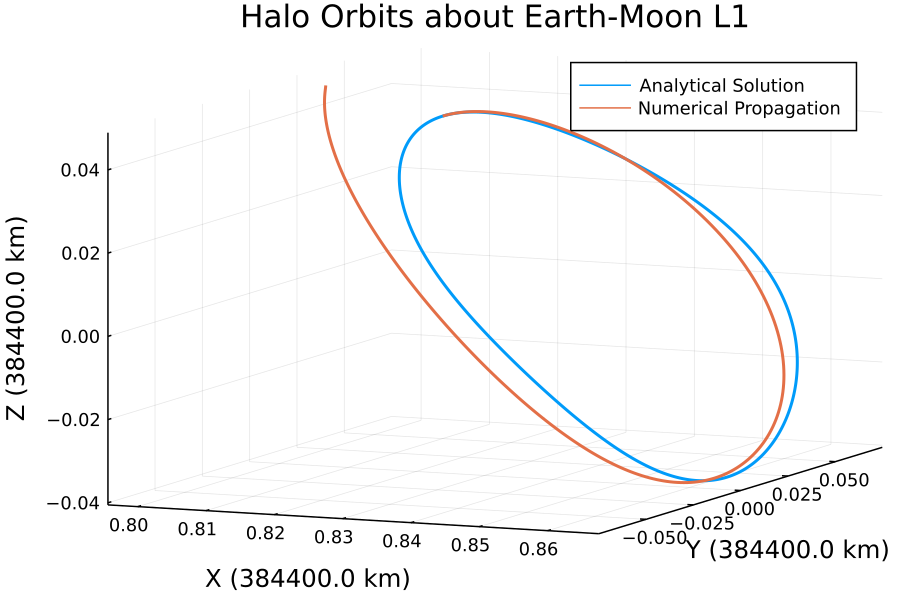
\includegraphics[width=0.5\textwidth]{analytical_propagation.png}
    \caption{Numerically propagated analytical solution}
\end{figure}

\subsection{Numerical Solution}

As shown previously, the analytical Halo orbit approximation is 
not numerically periodic when provided as an initial condition
to a numerical integrator. A differential correction scheme can 
be used to find a numerically periodic orbit within CR3BP dynamics, 
as described by Howell, summarized by Rund and Mireles, 
and implemented in private code written by Barbee, and
with publicly available notes and code by Mireles 
\cite{howell1984three} 
\cite{rund2018interplanetary}
\cite{barbeeCode}
\cite{mirelesNotes}
\cite{mirelesCode}.
There are several \textit{flavors} of this Newton-iteration correction algorithm. 
Each flavor \textit{typically} chooses two of the following initial condition
components to iterate on: $x_0$, $z_0$, $\dot{y}_0$, $\frac{T_0}{2}$.
Barbee's private Lyapunov orbit finding implementation chooses 
$\dot{y}_0$ and $\frac{T_0}{2}$ \cite{barbeeCode}.
Mireles' publicly available implementation chooses \textit{three} 
values: $z_0$, $\dot{y}_0$, and $\frac{T_0}{2}$ \cite{mirelesCode}. 
For this project, Mireles'
approach was combined with Barbee's Lyapunov orbit computation aproach. 
More detail about these flavors, and the differential
correction scheme more broadly, is provided in the remainder of this subsection. 

Broadly, the differential correction scheme works as follows.
Given an initial Halo orbit guess of the form provided by equations 
$\left(20\right)$ and $\left(21\right)$, and an initial Halo orbit
period $T_0$, propagate the orbit for $\frac{T_0}{2}$, and record
the final state transition matrix $\Phi$, 
Cartesian position $\overrightarrow{r}^{\star}$, 
velocity $\overrightarrow{v}^{\star}$, and acceleration
$\overrightarrow{a}^{\star}$. Here, we check if 
the final $x$-axis and $z$-axis velocities are within some tolerance of zero; 
$10^{-8}$ is one reasonable tolerance to use. If the final $x$-axis and $z$-axis
velocities are outside of your chosen tolerance, then a new Halo orbit
initial condition must be found. There are several differential correction 
options for refining your Halo orbit initial conditions. After 
applying one such method, and generating \textit{new} initial conditions, 
this process is repeated until some maximum number of iterations 
is reached, or final $x$-axis and $z$-axis velocities are successfully
within some tolerance of zero. 

\begin{align}
    \overrightarrow{r}^{\star} &= \begin{bmatrix} x_0 & 0 & z_0 \end{bmatrix} \\
    \overrightarrow{v}^{\star} &= \begin{bmatrix} 0 & \dot{y}_0 & 0 \end{bmatrix}
\end{align}

\subsubsection{Implementation used by Howell, Rund}
Howell presents two options, as shown in equations $\left(22\right)$ and 
$(23)$ \cite{howell1984three}. Equation $(22)$ iterates on the initial 
$z_0$ and $\dot{y}_0$ conditions, and equation $(23)$ iterates on the initial 
$x_0$ and $\dot{y}_0$ conditions. These corrections do not refine your 
$\frac{T_0}{2}$ guess, so they rely on your numerical integration stopping
when the orbit's $y$-axis component enters within some tolerance of zero;
this timepoint is the assumed half-period $\frac{T_0}{2}$ of the Halo orbit
at this iteration. Investigations as part of this project found this approach
problematic; approximate Halo orbit initial conditions produced by the 
previously discussed analytical algorithm may not cross the $X-Z$ plane in 
any reasonable time, and an arbitrary tolerance that doesn't 
produce "false positives" may be difficult to select. Still, others have 
implemented working versions of this particular algorithm. Rund summarized
this correction scheme, and used equation $(23)$ to calculate Halo orbit 
and invariant manifold results in a 2018 MS thesis \cite{rund2018interplanetary}.

\begin{equation}
\begin{aligned}
    F = & \left\{ 
        \begin{bmatrix} \Phi_{43} & \Phi_{45} \\ \Phi_{63} & \Phi_{65} \end{bmatrix} 
        - \frac{1}{\dot{y}_f} \begin{bmatrix} \ddot{x}_f \\ \ddot{z}_f \end{bmatrix} 
        \begin{bmatrix} \Phi_{23} & \Phi_{25} \end{bmatrix}\right\} \\
    & \hspace{1cm} \begin{bmatrix} z_0 \\ \dot{y}_0 \end{bmatrix} \leftarrow 
    \begin{bmatrix} z_0 \\ \dot{y}_0 \end{bmatrix} - F^{-1} \begin{bmatrix} \dot{x}_f \\ \dot{z}_f \end{bmatrix}
\end{aligned}
\end{equation}

\begin{equation}
\begin{aligned}
    F = & \left\{ 
        \begin{bmatrix} \Phi_{41} & \Phi_{45} \\ \Phi_{61} & \Phi_{65} \end{bmatrix} 
        - \frac{1}{\dot{y}_f} \begin{bmatrix} \ddot{x}_f \\ \ddot{z}_f \end{bmatrix} 
        \begin{bmatrix} \Phi_{21} & \Phi_{25} \end{bmatrix}\right\} \\
    & \hspace{1cm} \begin{bmatrix} x_0 \\ \dot{y}_0 \end{bmatrix} \leftarrow 
    \begin{bmatrix} x_0 \\ \dot{y}_0 \end{bmatrix} - F^{-1} \begin{bmatrix} \dot{x}_f \\ \dot{z}_f \end{bmatrix}
\end{aligned}
\end{equation}

\subsubsection{Implementation used by Barbee}
Barbee's Lyapunov orbit-finding MATLAB implementation uses a slightly 
different approach. Rather than refine $x_0$ and $\dot{y}_0$, his implementation
iterates on $\dot{y}_0$ and $\frac{T_0}{2}$ \cite{barbeeCode}. This approach 
works for Lyapnuov orbits: periodic orbits with $z \equiv 0$. The iteration 
of $\frac{T_0}{2}$ removes the reliance on accurate numerical integration 
terminal when $y$ reaches some tolerance of the $x-z$ plane; the integration 
can simply terminate when the current half-period guess, $\frac{T_0}{2}$, is 
reached. Investigations as part of this project found 
that correcting $\frac{T_0}{2}$, as opposed to relying on an integration 
termination condition to refine $\frac{T_0}{2}$, 
produces a far more robust orbit-finding 
implementation. Barbee's chosen initial condition refining 
approach is shown in equation $(24)$.

\begin{equation}
    \begin{aligned}
        F &= \begin{bmatrix} \Phi_{25} & \dot{y}_f \\ \Phi_{45} & \ddot{x}_f \end{bmatrix} \\
        \begin{bmatrix} \dot{y}_0 \\ \frac{T_0}{2} \end{bmatrix} & \leftarrow 
        \begin{bmatrix} \dot{y}_0 \\ \frac{T_0}{2} \end{bmatrix} - F^{-1} \begin{bmatrix} y_f \\ \dot{x}_f \end{bmatrix}
    \end{aligned}
\end{equation}

At this point, we've discussed three flavors of the periodic-orbit-finding 
differential correction algorithm. The first two implementations, 
as originally presented by Howell in \cite{howell1984three}, discussed 
do \textit{not} refine the half-period guess for the periodic orbit; this 
results in a potential implementation weakness when used in tandem with 
the analytical solution, as previously discussed. The third implementation,
as provided by Barbee in \cite{barbeeCode}, removes this weakness by 
correcting the half-period initial guess with each iteration. Still, Barbee's
implementation does not refine three-dimensional (Halo) orbit guesses.
Combining the best aspects of each flavor would allow for Lyapunov \textit{and}
Halo orbit computation, without relying on numerical integration
termination conditions. Mireles provides one such implementation in 
publicly available notes and code \cite{mirelesNotes} \cite{mirelesCode}.

\subsubsection{Implementation used by Mireles}
Mireles' implementation iterates on \textit{three} initial conditions:
$z_0$, $\dot{y}_0$, and $\frac{T_0}{2}$ \cite{mirelesNotes} \cite{mirelesCode}.
This approach to initial condition correction is shown in equation $(25)$.
Investigations as part of this project found that the approach described by 
equation $(25)$ is robust when applied to Halo orbit guesses provided 
by the previously discussed analytical solution. The implementation of this 
approach developed for this project failed to converge on numerically 
periodic Lyapunov (two-dimensional) orbits. This is likely a result 
of the $z_0$ iteration used. Lyapunov orbits have $z \equiv 0$ by definition, 
so an initial condition with $z_0 = 0$ would not produce any correction.
In other words, this scheme relies on using $z_0$ corrections to 
converge on a numerically periodic orbit. If $z \equiv 0$, then we've lost 
a degree of freedom for this correction algorithm. Next, one final 
implementation is provided that corrects this issue.

\begin{equation}
    \begin{aligned}
        F &= \begin{bmatrix} \Phi_{43} & \Phi_{45} & \ddot{x}_f \\
                             \Phi_{63} & \Phi_{65} & \ddot{z}_f \\
                             \Phi_{23} & \Phi_{25} & \dot{y}_f \end{bmatrix} \\
        \begin{bmatrix} z_0 \\ \dot{y}_0 \\ \frac{T_0}{2} \end{bmatrix} & \leftarrow 
        \begin{bmatrix}z_0 \\ \dot{y}_0 \\ \frac{T_0}{2} \end{bmatrix} - F^{-1} 
        \begin{bmatrix} \dot{x}_f \\ \dot{z}_f \\ y_f \end{bmatrix}
    \end{aligned}
\end{equation}

\subsubsection{General Implementation}
Recall that Howell presented two iteration options: one to refine $x_0$, and 
another to refine $z_0$. We can use this approach in combination with Mireles'
implementation to produce a general periodic orbit solver that works for both 
Lyapunov and Halo orbits. This approach is also discussed in Mireles' 
course notes \cite{mirelesNotes}. The general orbit solver implementation 
can use an \textit{if, else} block to check whether the initial condition 
is that of an approximate Lyapunov orbit ($z_0 = 0$), or a Halo orbit 
($z_0 \neq 0$). If the initial condition is an approximate Lyapunov orbit,
then equation $(26)$ should be used. Otherwise, investigations as part of this 
project found equation $(27)$ produced robust results. 

\begin{equation}
    \begin{aligned}
        F &= \begin{bmatrix} \Phi_{41} & \Phi_{45} & \ddot{x}_f \\
                             \Phi_{61} & \Phi_{65} & \ddot{z}_f \\
                             \Phi_{21} & \Phi_{25} & \dot{y}_f \end{bmatrix} \\
        \begin{bmatrix} x_0 \\ \dot{y}_0 \\ \frac{T_0}{2} \end{bmatrix} & \leftarrow 
        \begin{bmatrix} x_0 \\ \dot{y}_0 \\ \frac{T_0}{2} \end{bmatrix} - F^{-1} 
        \begin{bmatrix} \dot{x}_f \\ \dot{z}_f \\ y_f \end{bmatrix}
    \end{aligned}
\end{equation}

\begin{equation}
    \begin{aligned}
        F &= \begin{bmatrix} \Phi_{43} & \Phi_{45} & \ddot{x}_f \\
                             \Phi_{63} & \Phi_{65} & \ddot{z}_f \\
                             \Phi_{23} & \Phi_{25} & \dot{y}_f \end{bmatrix} \\
        \begin{bmatrix} z_0 \\ \dot{y}_0 \\ \frac{T_0}{2} \end{bmatrix} & \leftarrow 
        \begin{bmatrix}z_0 \\ \dot{y}_0 \\ \frac{T_0}{2} \end{bmatrix} - F^{-1} 
        \begin{bmatrix} \dot{x}_f \\ \dot{z}_f \\ y_f \end{bmatrix}
    \end{aligned}
\end{equation}

\subsection{Halo Orbit Results}
This final implementation (the combination of equations $(26)$ and $(27)$) 
is robust for Lyapunov \textit{and} Halo orbits about collinear Lagrange points. 
This implementation was impemented within \textit{GeneralAstrodynamics.jl}, and 
was used with the previously discussed analytical algorithm to generate 
periodic orbits for the remainder of this project \cite{carpinelli2020astro}.
The analytical algorithm takes physical orbit attributes as inputs: $z$-axis 
amplitude, phase angle, Lagrange point ($L1$ or $L2$), and hemisphere 
(northern, or southern) \cite{rund2018interplanetary}. 
The \textit{approximate} analytical solution generated 
with Richardson's analytical algorithm can then be used as an initial 
condition for the numerical algorithm \cite{rund2018interplanetary} 
\cite{richardson1980analytical}. When placed in series in this way, the 
analytical and numerical orbit-finding algorithms discussed so far form a 
kind of "black box"; the user specifies desired Halo orbit attributes, 
and the algorithms provide a numerically periodic Halo orbit initial condition.
\figurename{2} shows one result of the analytical and numerical algorithms 
working in tandem; the numerical algorithm found a periodic orbit \textit{nearby}
the approximate analytical solution. 

\begin{figure}[H]
    \hskip -0.3cm
    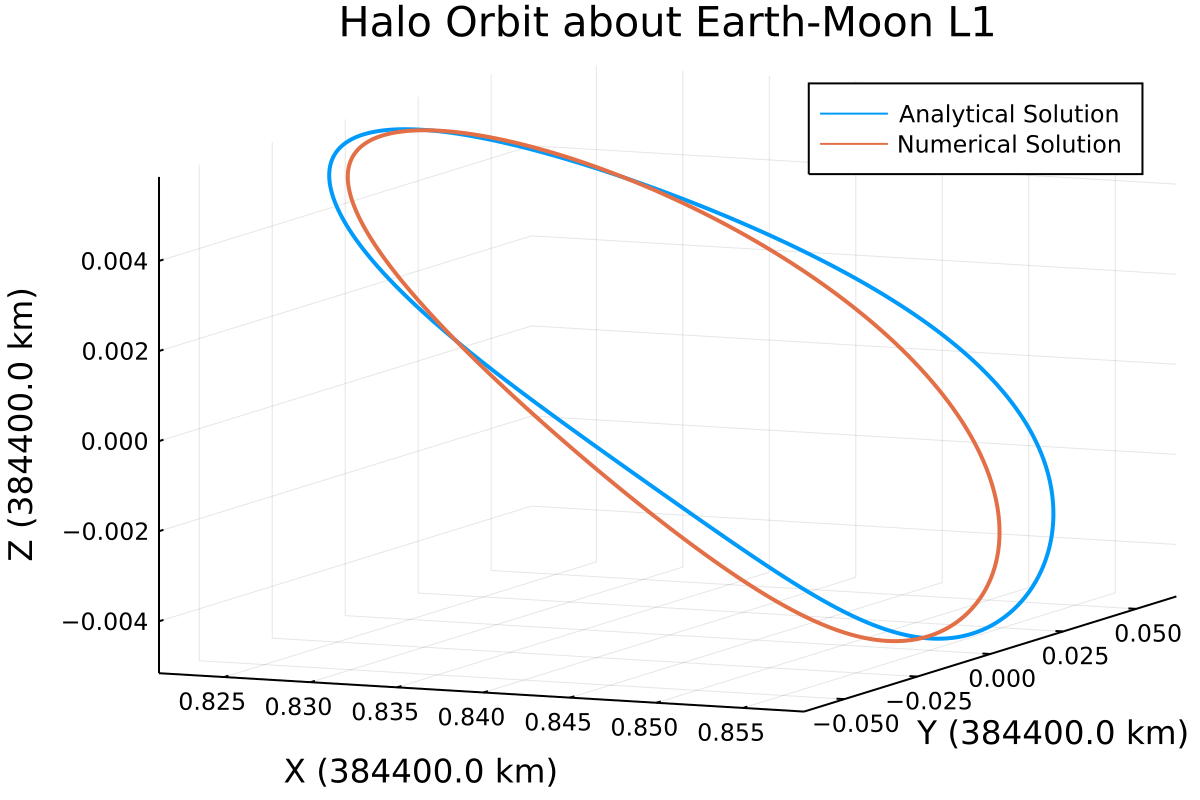
\includegraphics[width=0.5\textwidth]{analytical_numerical_halo.png}
    \caption{Analytical and Iterative Numerical solutions}
\end{figure}

While periodic orbits within CR3BP dynamics are catalogued in literature,
they can be difficult to find. A catalog of over $130,000$ periodic orbits 
within our solar system has been posted to GitHub as a collection of CSV files 
\cite{carpinelli2020halos}. The logged files are not optimized for disk 
space; they are instead optimized for clarity. Each row within the logged files 
provides normalized mass parameter, Lagrange point to orbit, Jacobi constant,
normalized $z$-axis amplitude, orbital period, and  
normalized, Synodic Cartesian states. Periodic orbits were catalogued for 
Sun-Venus, Sun-Earth, Earth-Moon, Sun-Mars, Sun-Jupiter, and Sun-Saturn CR3BP 
systems. A fraction of the computed Halo orbits are provided \tablename{1}.

A collection of periodic orbits can be computed with slightly varying 
$z$-axis amplitudes; this can be referred to as a family of Halo orbits
\cite{rund2018interplanetary}. 
Example families of periodic orbits within the Earth-Moon, Sun-Mars, 
and Sun-Jupiter systems are presented in \figurename{3}, \figurename{4},
and \figurename{5}. Note that both \figurename{4} and \figurename{5} 
look very similar because all orbits are plotted with nondimensional units.

In summary, several Halo orbit solvers have been pieced together to form 
a robust, open-source Julia implementation. This implementation produced 
all results presented so far, and was also used to explore invariant 
manifolds within CR3BP dynamics. The remainder of this paper summarizes
the existance of invariant manifolds, computational methods, 
applications in mission design, and methods and associated challenges 
in computing manifold-based interplanetary transfers. 

\end{multicols}
\newpage

\begin{landscape}
\begin{table}
\begin{tabular}{cccccccc}
    Mass Parameter & Lagrange Point & $Z$-Amplitude & Period & $x$ & $z$ & $\dot{y}$ \\
    $0.012150584269940356$ & $1.0$ & $0.0$ & $2.7536820171259744$ & $0.8222791805122408$ & $0.0$ & $0.13799313179964737$\\
    $0.012150584269940356$ & $1.0$ & $0.002$ & $2.7430279744649004$ & $0.8233905115990996$ & $0.0022207698036084363$ & $0.1264086161524851$\\
    $0.012150584269940356$ & $1.0$ & $0.004$ & $2.743129618348479$ & $0.8233893741253737$ & $0.004442307958743803$ & $0.12665484442364439$\\
    $0.012150584269940356$ & $1.0$ & $0.006$ & $2.743298907640046$ & $0.8233876253798795$ & $0.006665380456556792$ & $0.12706382260243482$\\
    $0.012150584269940356$ & $1.0$ & $0.008$ & $2.7435356656350174$ & $0.8233854825357569$ & $0.008890748615484967$ & $0.12763347860600016$\\
    $0.012150584269940356$ & $1.0$ & $0.01$ & $2.7438396430341294$ & $0.8233832430275673$ & $0.011119166862915583$ & $0.12836097250130557$\\
    $0.012150584269940356$ & $2.0$ & $0.001999$ & $3.4154785217654346$ & $1.1203619239893596$ & $0.001835091590818184$ & $0.17611109647933998$\\
    $3.003480593992993e-6$ & $1.0$ & $0.0$ & $3.057037166436106$ & $0.9889069589528534$ & $0.0$ & $0.008529372360506582$\\
    $3.003480593992993e-6$ & $1.0$ & $0.002$ & $3.0562630985504198$ & $0.9889296115452058$ & $0.0022759531712711633$ & $0.009571654363317172$\\
    $3.003480593992993e-6$ & $1.0$ & $0.004$ & $3.0408810610908192$ & $0.9891686188174361$ & $0.0046921863531775585$ & $0.011428450586881073$\\
    $3.003480593992993e-6$ & $1.0$ & $0.006$ & $2.9968780486251165$ & $0.9897509664037121$ & $0.007350439066516196$ & $0.013571383652713521$\\
    $3.003480593992993e-6$ & $1.0$ & $0.008$ & $2.8360875768267277$ & $0.9909674701532162$ & $0.010323704902503393$ & $0.015198885580121493$\\
    $3.003480593992993e-6$ & $2.0$ & $0.001798$ & $3.09794993304811$ & $1.0080662252502852$ & $0.001672550237255738$ & $0.010798428273484711$\\
    $3.003480593992993e-6$ & $2.0$ & $0.003798$ & $3.0755344619414036$ & $1.0068608443606484$ & $0.0035047324922114834$ & $0.014513397367974044$\\
    $3.2271548760451657e-7$ & $1.0$ & $0.0$ & $3.067790305289647$ & $0.9947153604918691$ & $0.0$ & $0.004052940170205446$\\
    $3.2271548760451657e-7$ & $1.0$ & $0.0001$ & $3.0713331541226148$ & $0.9946990969840135$ & $0.00011259909689815706$ & $0.00420141728779284$\\
    $3.2271548760451657e-7$ & $1.0$ & $0.0002$ & $3.071197879663506$ & $0.9946998314896827$ & $0.0002252842583036334$ & $0.004214196175484041$\\
    $3.2271548760451657e-7$ & $1.0$ & $0.0003$ & $3.0709713120763475$ & $0.9947010768650656$ & $0.00033814100956578$ & $0.004235364341723893$\\
    $3.2271548760451657e-7$ & $1.0$ & $0.0004$ & $3.0706517674163125$ & $0.9947028642521663$ & $0.00045125381930966155$ & $0.004264731532729223$\\
    $3.2271548760451657e-7$ & $1.0$ & $0.0005$ & $3.070236850446078$ & $0.9947052359932343$ & $0.0005647056232279373$ & $0.004302040405811711$\\
    $3.2271548760451657e-7$ & $1.0$ & $0.0006$ & $3.069723416205373$ & $0.9947082444991275$ & $0.0006785774056064239$ & $0.004346974627389325$\\    
    $0.0009536838895767626$ & $1.0$ & $0.0$ & $2.9370190457587504$ & $0.9253021269565835$ & $0.0$ & $0.0585266341496578$\\
    $0.0009536838895767626$ & $1.0$ & $0.002$ & $2.9354795531765805$ & $0.9253921878089174$ & $0.0022382733013625957$ & $0.05785899301066716$\\
    $0.0009536838895767626$ & $1.0$ & $0.004$ & $2.9354974958876$ & $0.9254047001045744$ & $0.004480217902893781$ & $0.05829041425456174$\\
    $0.0009536838895767626$ & $1.0$ & $0.006$ & $2.9355234346153742$ & $0.9254269085233069$ & $0.006729454676907429$ & $0.05899947503986548$\\
    $0.0009536838895767626$ & $1.0$ & $0.008$ & $2.935551270469769$ & $0.9254607390135051$ & $0.008989508064503429$ & $0.059972051406433184$\\
    $0.0009536838895767626$ & $1.0$ & $0.01$ & $2.935572154787768$ & $0.9255086965138954$ & $0.011263768116134604$ & $0.06118987977165465$\\
    $0.0009536838895767626$ & $2.0$ & $0.001999$ & $3.223538695196383$ & $1.0560878711527533$ & $0.001854944179107667$ & $0.07004521113569465$\\    
\end{tabular}
\caption{Periodic Orbits within the Earth-Moon, Sun-Earth, Sun-Mars, and Sun-Jupiter Systems}
\end{table}
\end{landscape}

\newpage
\begin{multicols}{2}

\begin{figure}[H]
    \hskip -0.3cm
    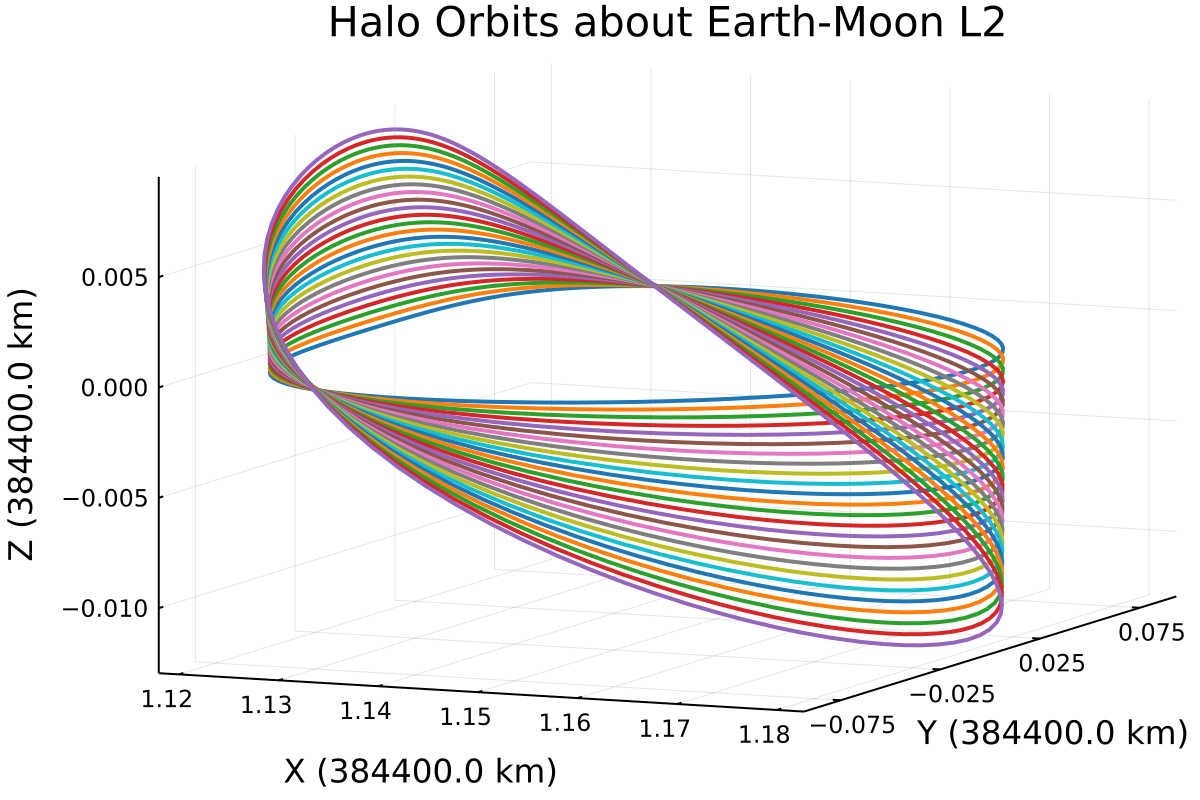
\includegraphics[width=0.5\textwidth]{halo_family.png}
    \caption{Famly of Halo orbits about Earth-Moon L2}
\end{figure}

\begin{figure}[H]
    \hskip -0.3cm
    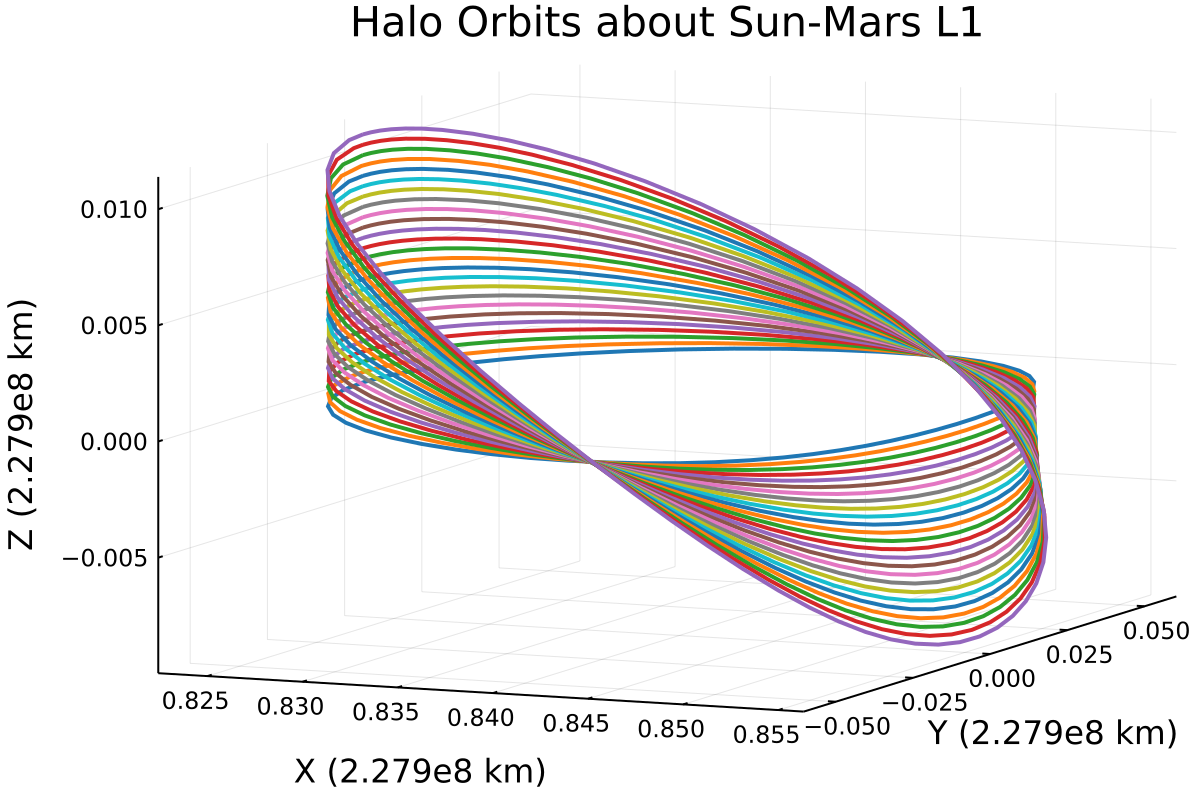
\includegraphics[width=0.5\textwidth]{halo_family_sm1.png}
    \caption{Famly of Halo orbits about Sun-Mars L1}
\end{figure}

\begin{figure}[H]
    \hskip -0.3cm
    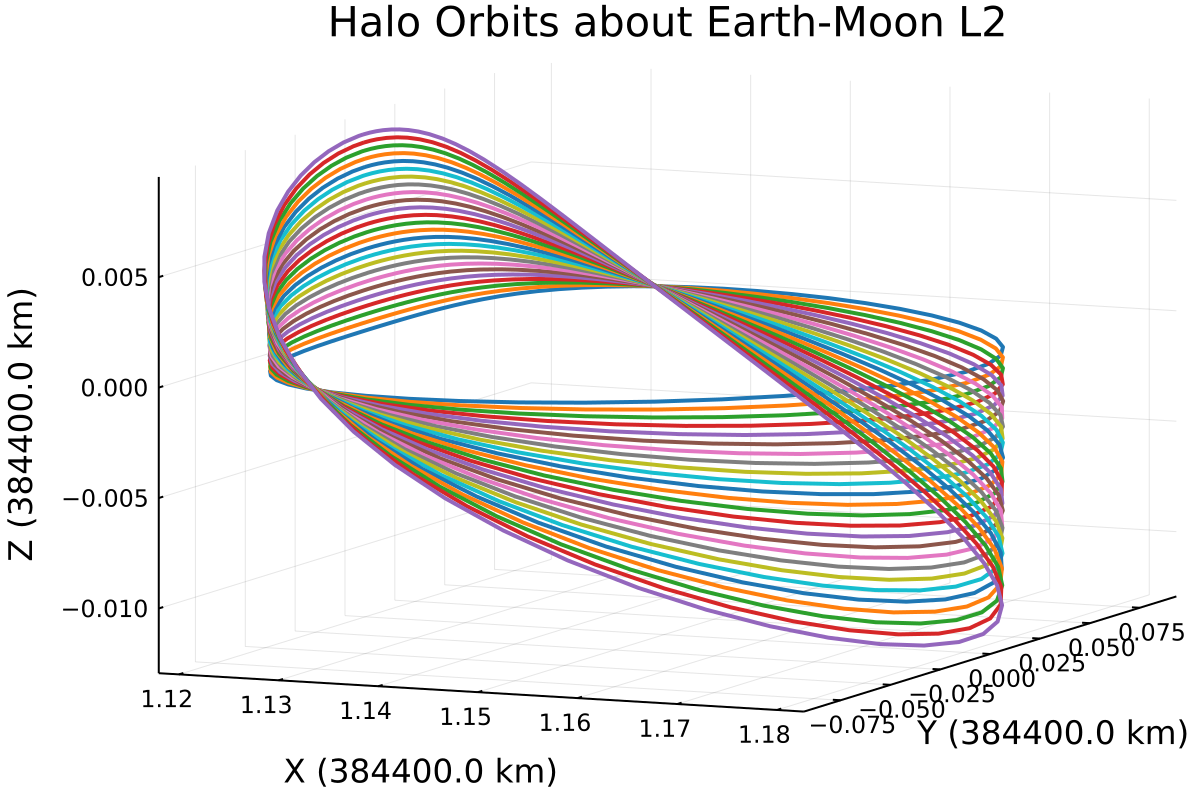
\includegraphics[width=0.5\textwidth]{halo_family_sj1.png}
    \caption{Famly of Halo orbits about Sun-Jupiter L1}
\end{figure}

\section{Invariant Manifolds}

Before discussing invariant manifolds, a brief discussion of 
general nonlinear dynamics may be helpful. 

\subsection{Nonlinear Dynamics Review}
Lagrange points 
are the equilibrium points of the nonlinear CR3BP dynamics.
The phase space around these Lagrange points will have stability 
characteristics, e.g. stable focus, unstable focus, and
saddle point behavior. As discussed in the preceding sections, the phase
space around Lagrange points can also feature periodic orbits, e.g. 
Lyapunov and Halo orbits. Once again, similar to any nonlinear 
dynamical system, the Jacobian of a CR3BP state vector is the 
local linearization of the CR3BP dynamics evaluated at that particular 
state vector. We can use the local linearization to characterize the 
stability properties of the dynamics at that point in the phase space, 
and points along periodic orbits are no exception. States 
along periodic orbits can benefit from some reduced computational 
expense by using the Monodromy matrix, $M$ \cite{rund2018interplanetary}. 
We can find $M$ by 
propagating a periodic orbit's initial conditions for one period, 
with the dynamics of the state transition matrix included. The 
state transition matrix should be initialized to a $6 \times 6$ 
identity matrix at the start of the numerical integration. 
The final state transition matrix in this propagation is the 
Monodromy matrix, and we can use this matrix to 
evaluate local linear modes at each point along the periodic 
orbit, as opposed to computing the state transition matrix at each point 
we wish to evaluate. 

\subsection{Calculating Invariant Manifolds}
Invariant manifolds within CR3BP dynamics are tubes of trajectories
that converge to, or diverge from, periodic orbits or Lagrange points
\cite{rund2018interplanetary} \cite{topputo2005low}. The term 
\textit{manifold} comes from their three-dimensional, surface-like
shapes. The term \textit{invariant} applies because, once placed in 
a manifold, a spacecraft governed by CR3BP dynamics
will stay in that manifold for all time (without external forces applied).

For this project, invariant manifolds about Halo orbits were 
explored. A spacecraft on a periodic orbit can be perturbed 
onto a trajectory within a manifold by perturbing the 
state vector in the direction of the Mondomy matrix's stable 
or unstable eigenvectors. Each Monodromy matrix should have 
two real eigenvalues, and two pairs of complex eigenvalues.
The smaller real eigenvalue should be less than one,
and the larger real eigenvalue should be greater than one 
\cite{gomez2001dynamicsv1}. As an additional check, 
the pair of real eigenvalues should also be multiplicative 
inverses of one another \cite{mirelesNotes}. The eigenvector 
of the Monodromy matrix that is associated with the 
larger real eigenvalue is the unstable eigenvector $V^U$, and 
the eigenvector associated with the smaller real eigenvalue is 
the stable eigenvector $V^S$ \cite{rund2018interplanetary}.
Equations $(28)$, $(29)$, $(30)$, $(31)$, and $(32)$ describe 
the perturbation required to move from a periodic orbit 
onto the orbit's stable manifold $X^S$, or unstable manifold $X^U$;
all are pulled from Rund's thesis, and were also presented 
in a previous paper \cite{rund2018interplanetary} \cite{carpinelli2020halos}.

\begin{equation}
    V_i^{S} = \Phi(t_0 + t_i, t_0) V^S
\end{equation}
\begin{equation}
    V_i^{U} = \Phi(t_0 + t_i, t_0) V^U
\end{equation}
\begin{equation}
    X_i^{S} = X_i \pm \epsilon \frac{V_i^S}{|V_i^S|}
\end{equation}
\begin{equation}
    X_i^{U} = X_i \pm \epsilon \frac{V_i^U}{|V_i^U|}
\end{equation}

\begin{equation}
M = \Phi(t_0 + T, t_0)
\end{equation}

\begin{figure}[H]
    \hskip -0.3cm
    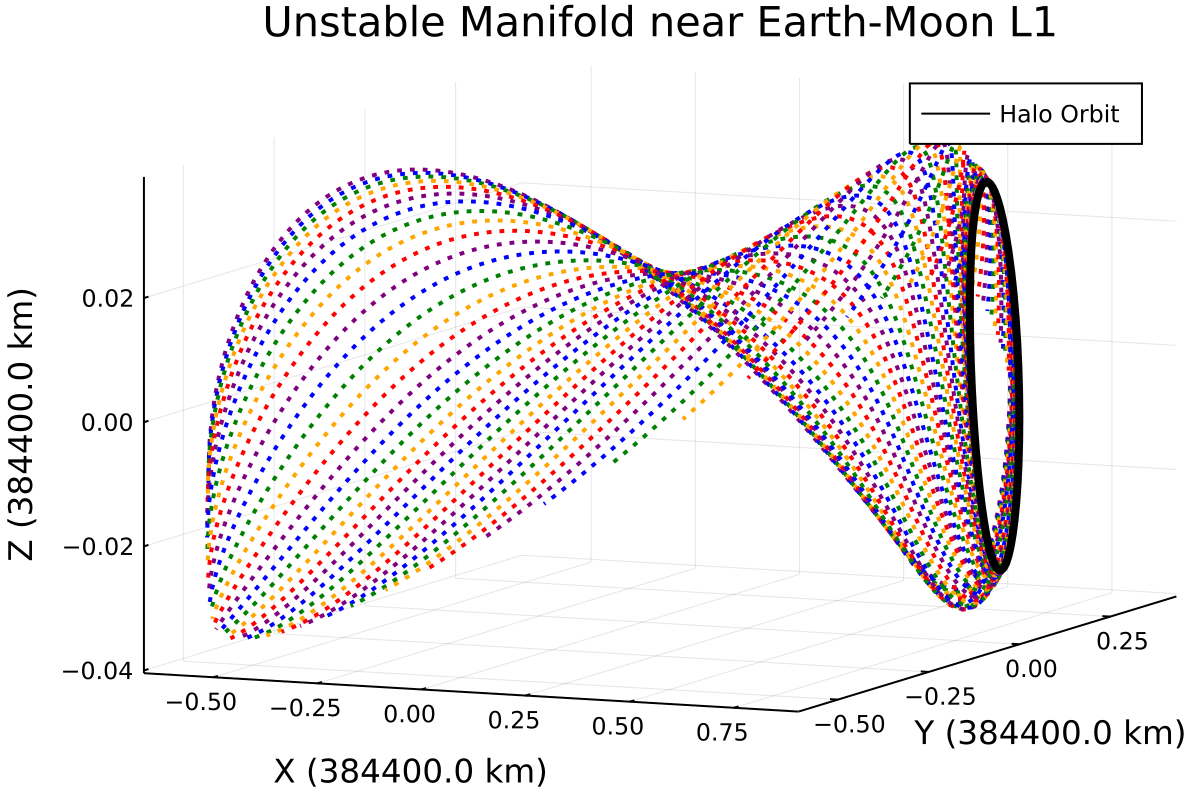
\includegraphics[width=0.5\textwidth]{unstable_manifold.png}
    \caption{Unstable Manifold near Earth-Moon L1}
\end{figure}

\section{Manifold-based Transfers}

\textit{
    An algorithm for using invariant manifolds to 
    design interplanetary transfers will be presented,
    as summarized by Rund \cite{rund2018interplanetary}.
    A Julia implementation will (hopefully!) be presented
    here as well.
}

\begin{figure}[H]
    \hskip -0.3cm
    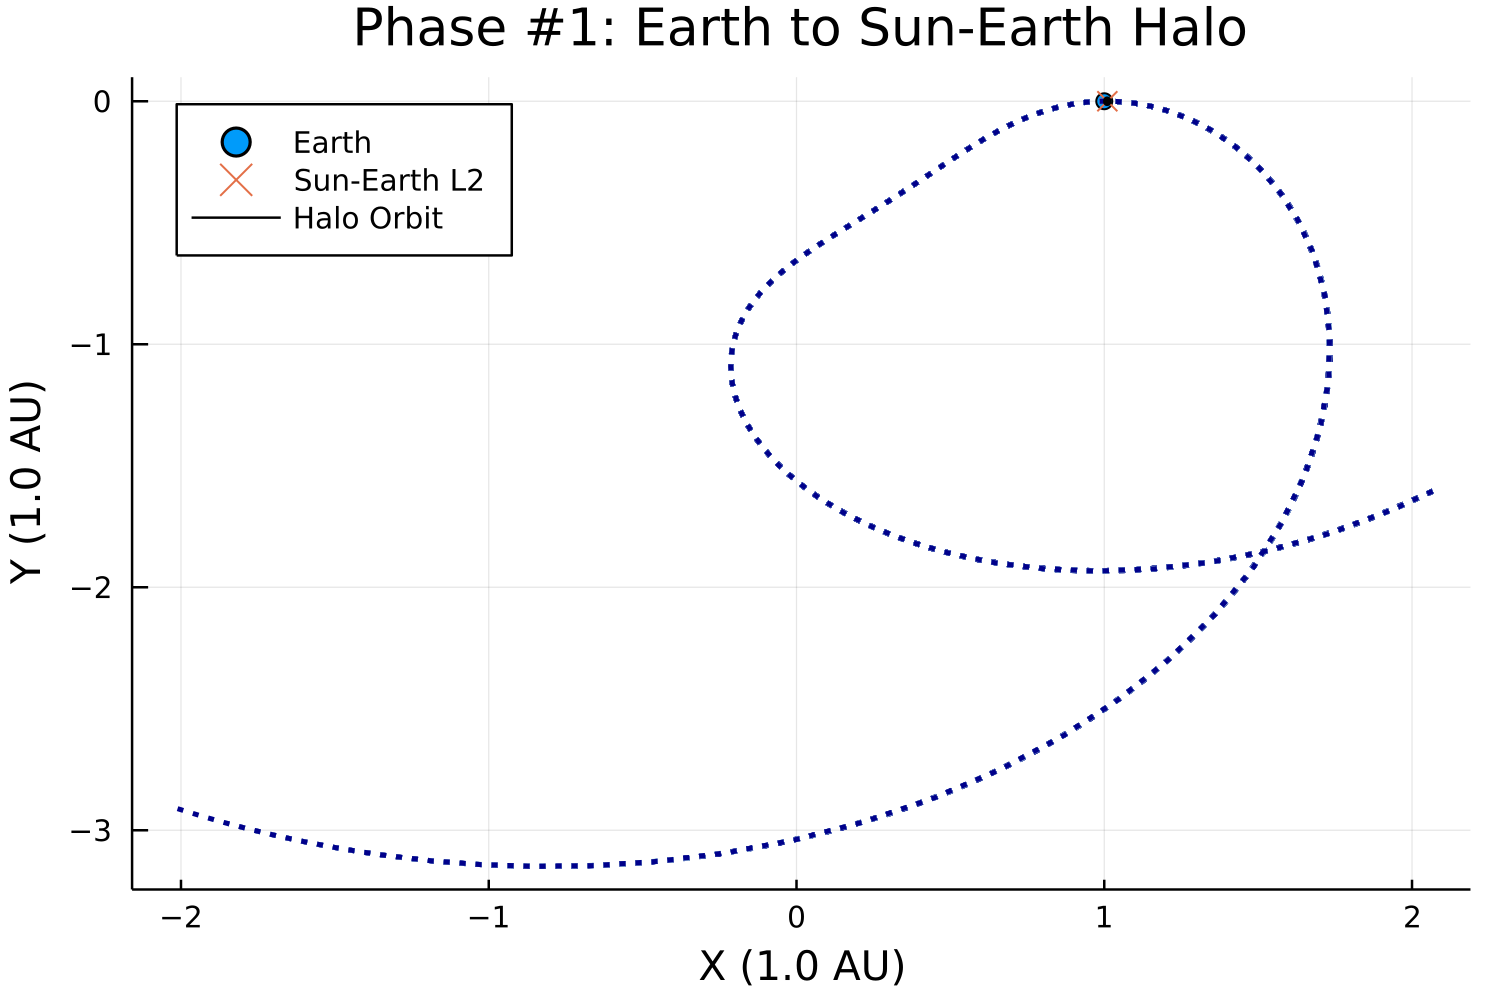
\includegraphics[width=0.5\textwidth]{manifold_transfer_phase1.png}
    \caption{Launch from Earth to Stable Manifold}
\end{figure}

\begin{figure}[H]
    \hskip -0.3cm
    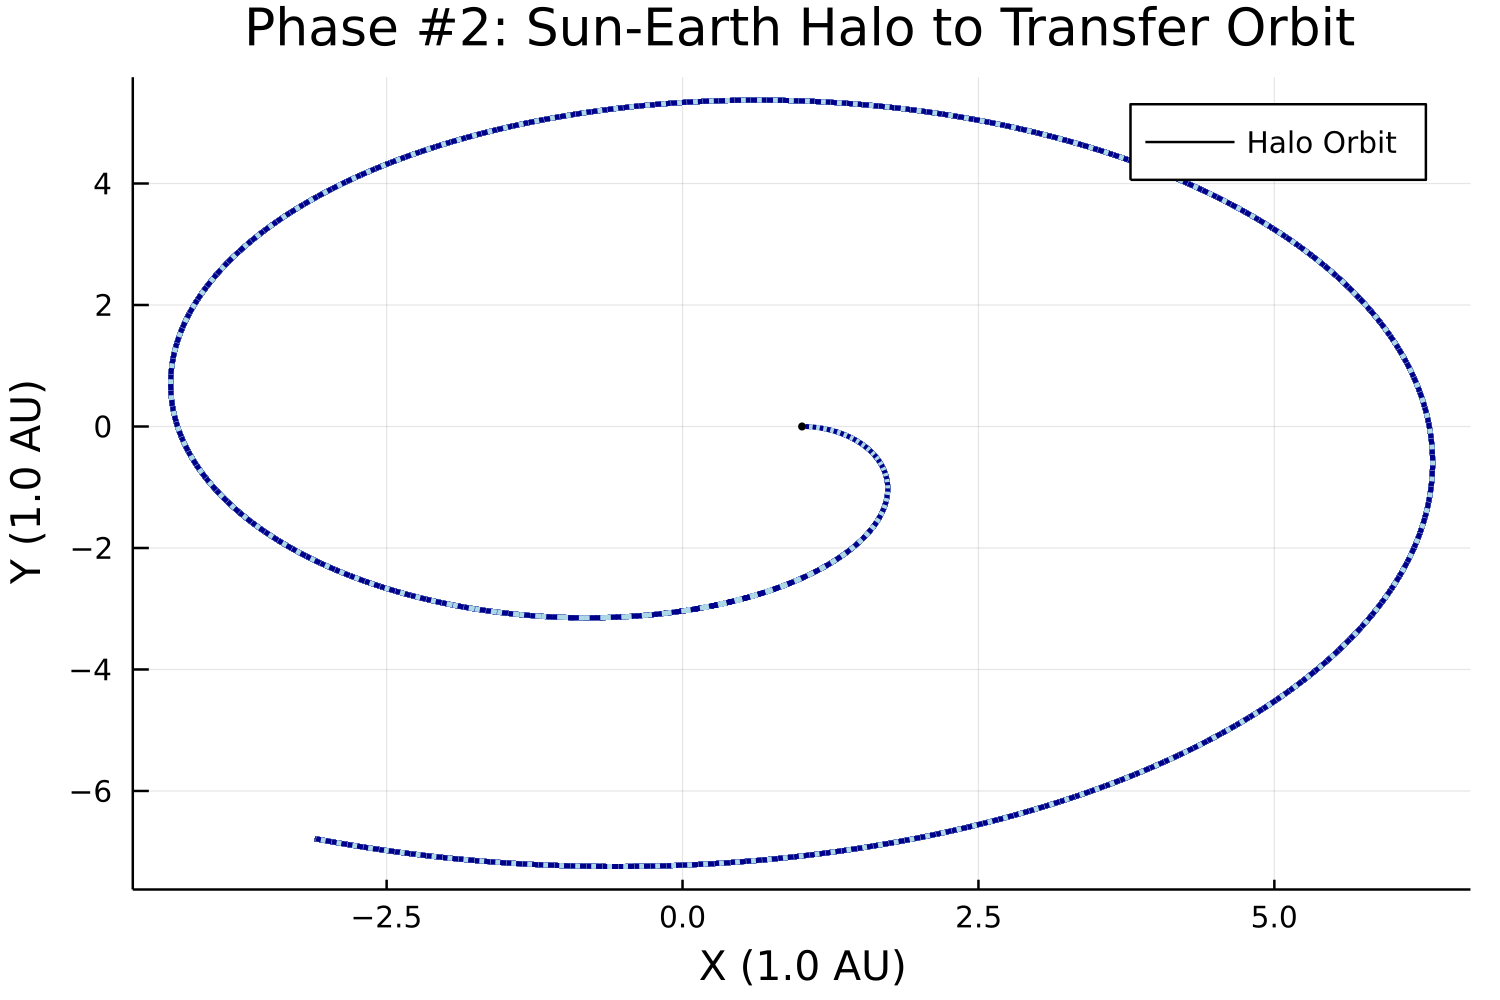
\includegraphics[width=0.5\textwidth]{manifold_transfer_phase2.png}
    \caption{Perturb Spacecraft onto Sun-Earth Unstable Manifold}
\end{figure}

\begin{figure}[H]
    \hskip -0.3cm
    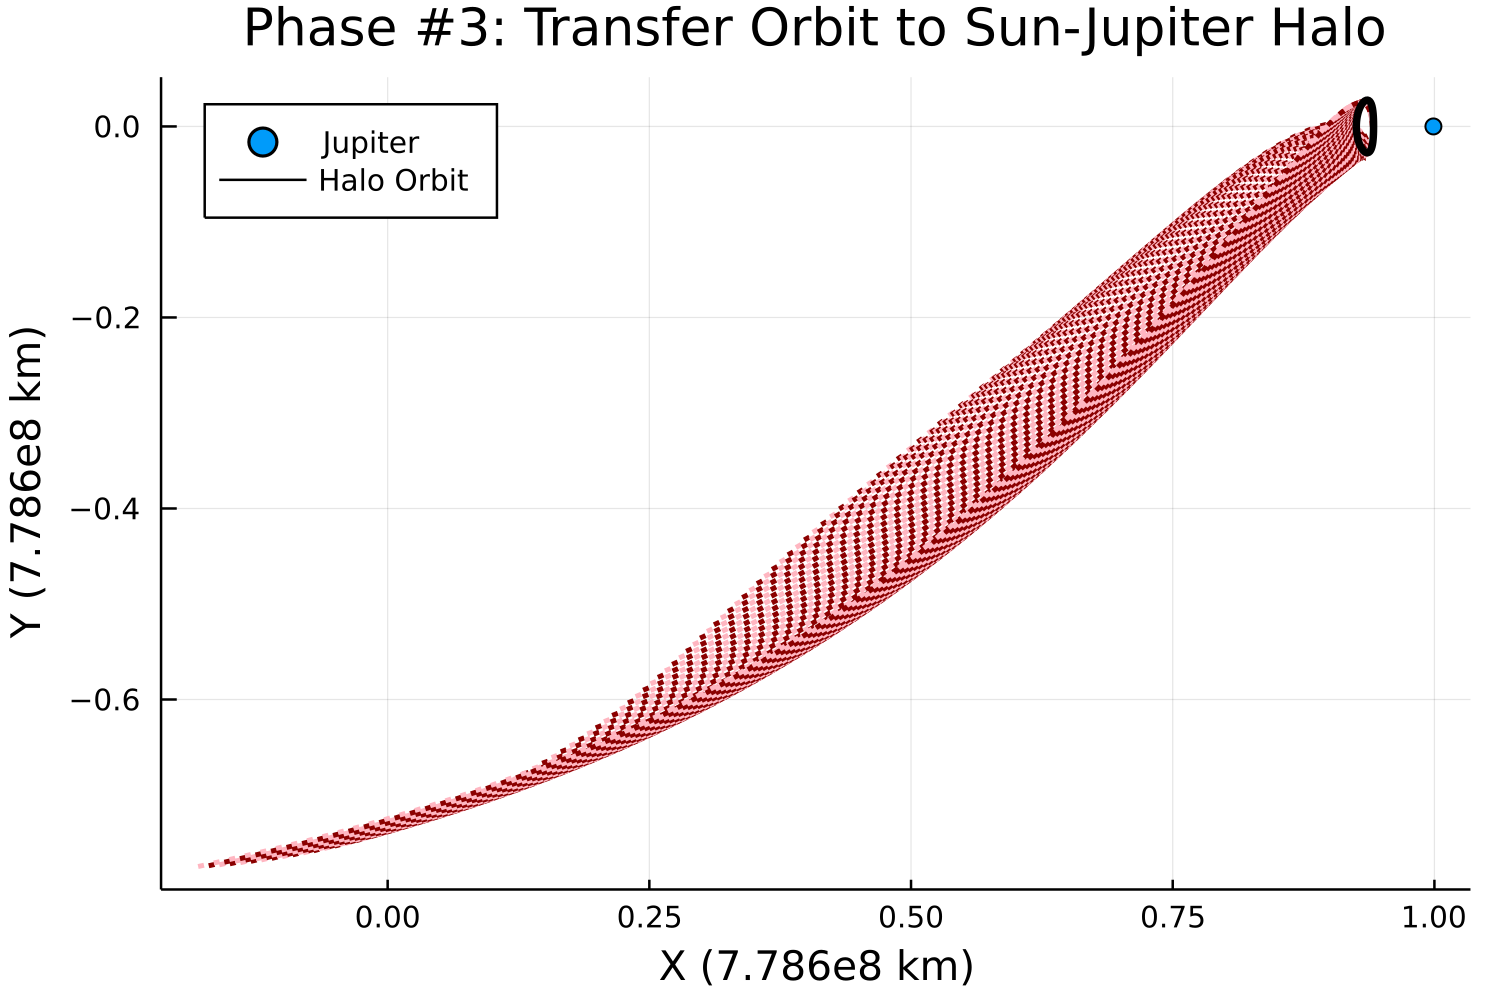
\includegraphics[width=0.5\textwidth]{manifold_transfer_phase3.png}
    \caption{Maneuver Spacecraft onto Sun-Jupiter Stable Manifold}
\end{figure}

\section{Conclusion}

\section{References}
\nocite{*}
\renewcommand\refname{\vskip -0.9cm}
\bibliography{sources}

\section{Appendix}
\textit{
    Will present all source code necessary to replicate 
    this project, including copy-pasted GeneralAstrodynamics.jl
    code that is available on GitHub. Any MATLAB implementations 
    will also be provided here, as MATLAB is a far more common 
    tool used by astrodynamics students. 
}

\end{multicols}

\end{document}